%%%%%%%%%%%%%%%%%%%%%%%%%%%%%%%%%%%%%%%%%%%%%%%%%%%%%%%%%%%%%%%%%%%%%%
%%	Name: "Signal analysis template"
%%	File name: signalanalysis_template_main
%%	Version: 1.5
%%
%%	Compiler: XeLaTeX
%%
%%%%%%%%%%%%%%%%%%%%%%%%%%%%%%%%%%%%%%%%%%%%%%%%%%%%%%%%%%%%%%%%%%%%%%

\documentclass[conference,compsoc,onecolumn]{IEEEtran}

% *** LANGUAGE UTILITY PACKAGES ***
\usepackage[utf8]{inputenc} % Required for including letters with accents
\usepackage[spanish]{babel}
\usepackage{multicol}
\usepackage{subcaption}

% *** USED PACKAGES ***
% *** MISC UTILITY PACKAGES ***
\usepackage{comment}			% Agregar comentarios
\usepackage{lipsum}				% Inserts dummy text
\usepackage{blindtext}
\usepackage{listings}					% Coding
\usepackage{verbatim}				% Verbatim
\usepackage[final]{pdfpages}
\usepackage{booktabs,dcolumn}
\usepackage{pdflscape}
\usepackage{afterpage}
%\setlist[itemize]{noitemsep, nolistsep}
\usepackage[bookmarks=false]{hyperref}
\usepackage{tcolorbox}									% Coloured boxes, for LATEX examples and theorems, etc
\usepackage{color}
\usepackage{xcolor} % Required for specifying colors by name									% Color packages foreground and back­ground color man­age­men
% *** CITATION PACKAGES ***
\usepackage{cite}
% *** GRAPHICS RELATED PACKAGES ***
\usepackage{graphicx}
\usepackage{caption}
\usepackage{subcaption}
\usepackage{pgfplots}
\usepackage{tikz}
\usetikzlibrary{shapes,arrows}
\usetikzlibrary{decorations.pathmorphing} % noisy shapes
\usetikzlibrary{fit}					% fitting shapes to coordinates
\usetikzlibrary{backgrounds}	% drawing the background after the foreground
\pgfplotsset{compat=1.13}
% *** MATH PACKAGES ***
\usepackage{amsmath}
\usepackage{mathtools}
\usepackage{amssymb}
\usepackage{amsfonts}
\usepackage{expl3}
\usepackage{bm}

% *** SPECIALIZED LIST PACKAGES ***
\usepackage{algorithmic}
\usepackage{listings}					% Coding
\usepackage[framed,numbered,autolinebreaks,useliterate]{mcode}
% *** ALIGNMENT PACKAGES ***
\usepackage{array}
% *** SUBFIGURE PACKAGES ***
%\ifCLASSOPTIONcompsoc
%\usepackage[caption=false,font=normalsize,labelfont=sf,textfont=sf]{subfig}
%\else
%\usepackage[caption=false,font=footnotesize]{subfig}
%\fi
% *** FLOAT PACKAGES ***
\usepackage{fixltx2e}
\usepackage{stfloats}
%\fnbelowfloat
%\usepackage{dblfloatfix}
% *** PDF, URL AND HYPERLINK PACKAGES ***
\usepackage{url}
\usepackage{everypage}


\usepackage{multirow} % In order to be able to insert rows spanning multiple lines
\usepackage{verbatim}
\usepackage[all]{xy}
\usepackage{listings}
\usepackage{multibib}
\usepackage{setspace} 
\usepackage{algorithm}			    	  % To insert nice algorithms

% *** CARPETA DONDE SE GUARDARAN LAS IMAGENES ***
\graphicspath{{figures/}}

% *** NUEVOS COMANDOS Y CONFIGURACIONES VARIAS ***
\interdisplaylinepenalty=2500
\newcommand{\Lpagenumber}{\ifdim\textwidth=\linewidth\else\bgroup
	\dimendef\margin=0
	\ifodd\value{page}\margin=\oddsidemargin
	\else\margin=\evensidemargin
	\fi
	\raisebox{\dimexpr -\topmargin-\headheight-\headsep-0.5\linewidth}[0pt][0pt]{%
		\rlap{\hspace{\dimexpr \margin+\textheight+\footskip}%
			\llap{\rotatebox{90}{\thepage}}}}%
	\egroup\fi}

\AddEverypageHook{\Lpagenumber}%

\newcommand{\newtxt}[1]{\textcolor{black}{#1}}
\renewcommand\IEEEkeywordsname{Palabras cláve:}
\newcommand{\mx}[1]{\mathbf{\bm{#1}}} % Matrix command
\newcommand{\vc}[1]{\mathbf{\bm{#1}}} % Vector command

%% Separación de palabras
\hyphenation{op-tical net-works semi-conduc-tor HHMMSS}

\begin{document}

% *** TITLES AND NAMES ***
% title of the document
\title{Entrega Proyecto 
}

\author{\IEEEauthorblockN{Sergio Rodriguez}
\IEEEauthorblockA{\textit{Ingeniería electrónica} \\
\textit{Universidad Sergio Arboleda}\\
sergio.rodriguez01@correo.usa.edu.co}
\and
\IEEEauthorblockN{Juan Sanchez}
\IEEEauthorblockA{\textit{Ingeniería electrónica} \\
\textit{Universidad Sergio Arboleda}\\
juan.sanchez03@correo.usa.edu.co}
}

\maketitle

\begin{abstract}
Por medio del presente proyecto se quiere ordenar verificar la cantidad de personas que estan contagiadas a nivel nacional en colombia de tal forma que se permita ver los datos de una forma mas organizada y global lo cual permita analizar la cantidad de contagiados y proporcionar informacion para una solucion de mejora encuanto a estos datos.
    
\end{abstract}

\begin{IEEEkeywords}
Covid-19, Graficos, Datos, Contagios 
\end{IEEEkeywords}

\section{Introducción}
Se desear poder ver, organizar y encontrar en el presente proyecto los datos sobre los contagios del covid en colombia a nivel nacional visto desde cada departamento por medio de graficas que nos permitan de alguna forma analizar los contagios de los hombres y las mujeres que hay en colombia por cada departamento por medio de la plataforma python que con las heramientas que este programa proporciona la facilidad de una  organizacon de los datos y asi mismo la grafica de los contagios por departamento.

\section{Marco teorico}

\textbf{Base de datos}: Por medio de datos.gov.co \cite{CovidColombia} se proporciona la informacion requerida para poder saber ucantos son los contagiados en diferentes departamentos, la base de datos es muy precisa ya que no solo anunci alos contagios sino tambien las notificaciones de las persnas que dicen estar contagiados sin estar seguro de eso, proporciona fecha, lugar , gener, de tal manera que facilita la grafica y los datos sobre los contagiados de tal manera que facilita el trabajo.\\

\textbf{Api rest}:  Por medio de esto el api rest es un sistema de productos y servicios que permite la comunicacion de los mismos sin la necesidad de saber como implementarlos , esto otorga la simplicidad y agilidad a la hora de diseñar o asi mismo de administrar.\\

\section{Resultados }

\begin{figure}[h!]
    \centering
    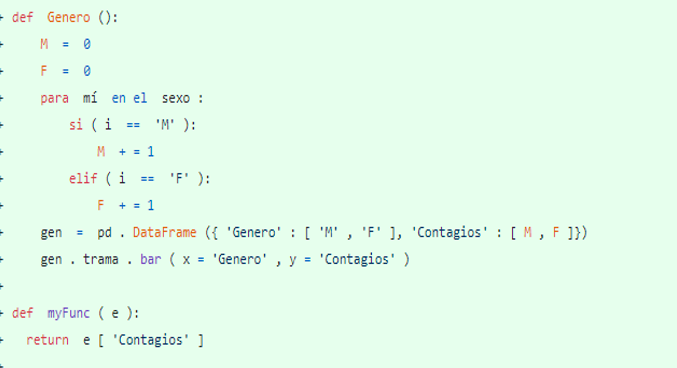
\includegraphics[scale=0.4]{images/i1.png}
    \caption{codigo para generar grafica por genero a nivel nacional .}
    \label{fig:fig1}
\end{figure}

Por medio de la figura1 se uede ver el codigo para lograr el funcionamiento de una grafica con la base de datos de os contgiados de tal manera que se exprese graficamente por 2 columnas en la grafica, una donde muestre los contagios de los hombres y otro de las mujeres a nivel nacional y no por departamento.\\


\begin{figure}[h!]
    \centering
    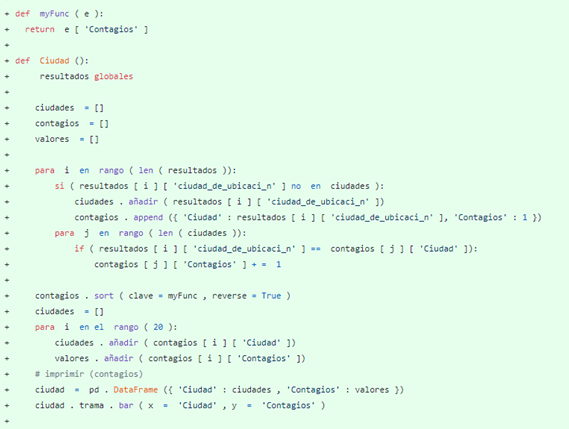
\includegraphics[scale=0.4]{images/i2.png}
    \caption{codigo para generar grafica por departamento de bogota nacional.}
    \label{fig:fig1}
\end{figure}

\begin{figure}[h!]
    \centering
    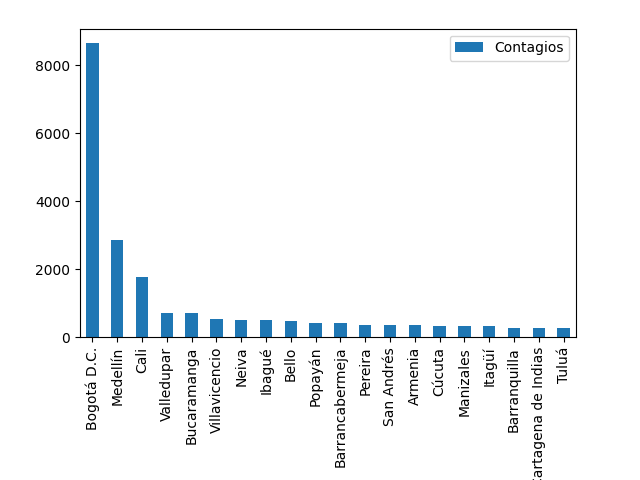
\includegraphics[scale=0.4]{images/Contagios_Por_Ciudad.png}
    \caption{Grafica de contagios por ciudad.}
    \label{fig:fig1}
\end{figure}

En la figura \ref{fig:barrasCiudad} se puede ver la grafica de los contagios por ciudad lo cual por medio del codigo presente en la figura numero dos se puede ver como se analiza la ciudad y se presenta por medio de la grafica lo contagios y numero de ellos presente.\\

\begin{figure}[h!]
    \centering
    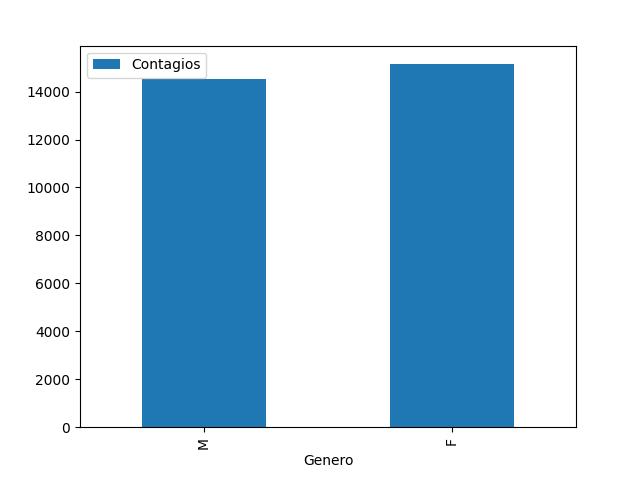
\includegraphics[scale=0.4]{images/Contagios_Por_Genero.png}
    \caption{Grafica de contagios por genero.}
    \label{fig:barrasCiudad}
\end{figure}

En la figura 4 se encuentra la grafica de los contagios por genero a nivel nacional con ayuda del codigo que esta en la figura 2 se llega a la organizacion de todos los contagios a nivel nacional de tal forma que los datos se organizan de tal manera que en la grafica estan representados los contagios por genero.\\ 

\begin{figure}[h!]
    \centering
    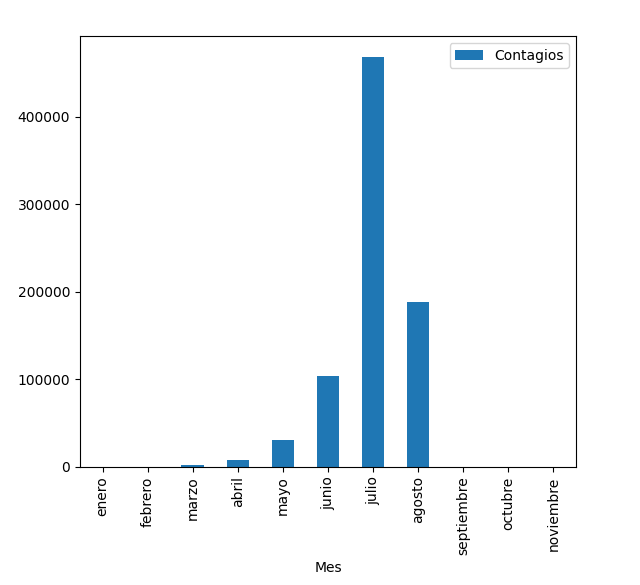
\includegraphics[scale=0.4]{images/Contagios_Por_Mes.png}
    \caption{Grafica de contagios por mes .}
    \label{fig:fig1}
\end{figure}

\begin{figure}[h!]
    \centering
    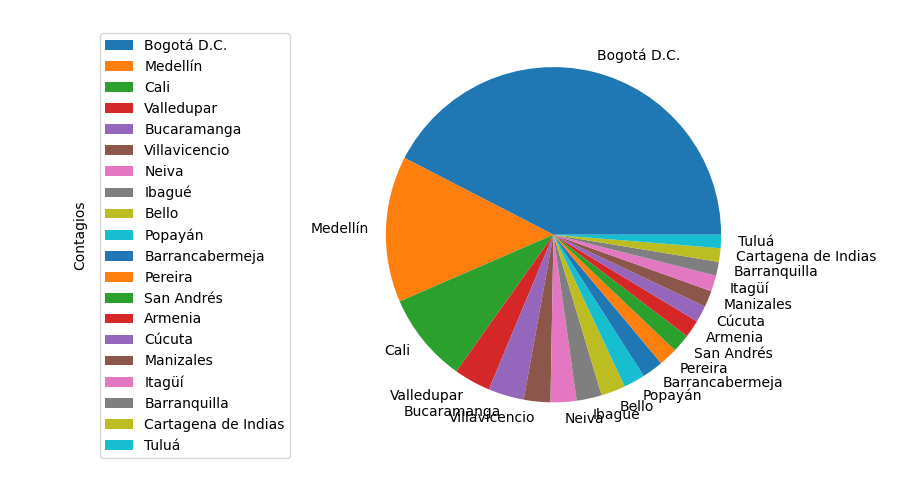
\includegraphics[scale=0.4]{images/Contagios_Por_ciudad_torta.png}
    \caption{Grafica de contagios por cuidad en  torta.}
    \label{fig:fig1}
\end{figure}

En la figura 5 se puede ver los contagios por mes del pais de colombia a medida que pasa el tiempo desde que llego la enfermedad al país.\\

\begin{figure}[h!]
    \centering
    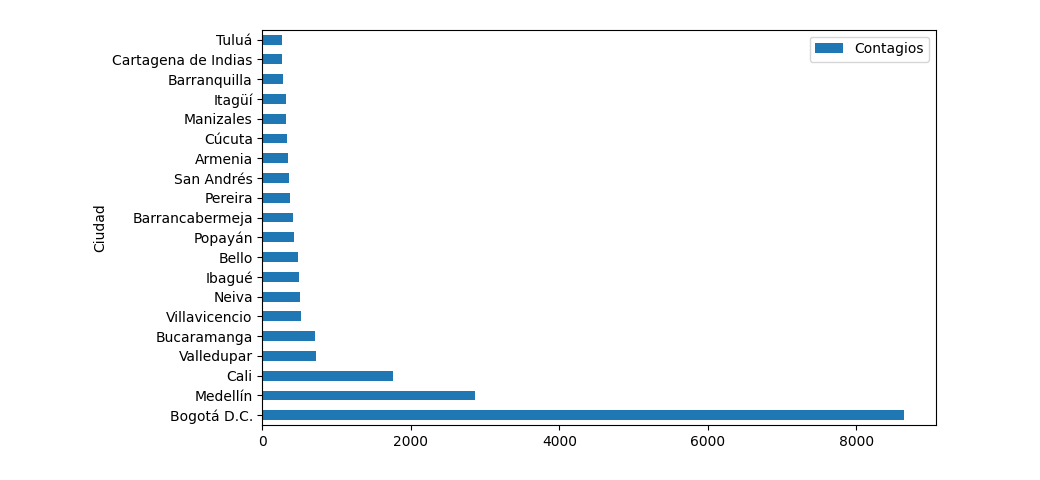
\includegraphics[scale=0.4]{images/Contagios_ciudad_barh.png}
    \caption{Grafica de contagios por cuidad en barh.}
    \label{fig:fig1}
\end{figure}

\begin{figure}[h!]
    \centering
    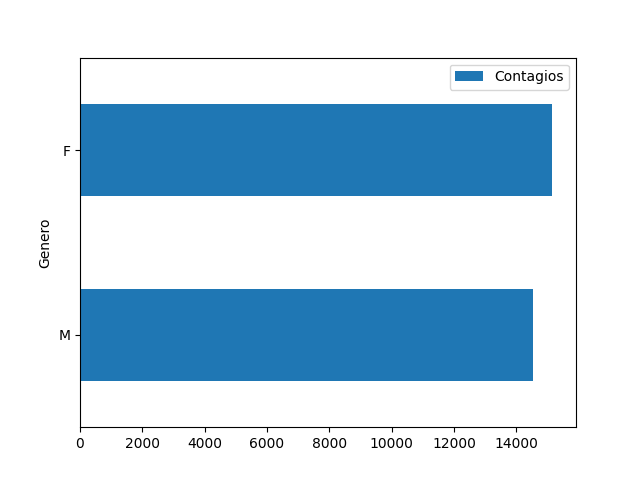
\includegraphics[scale=0.4]{images/Contagios_genero_barh.png}
    \caption{Grafica de contagios por genero en barh.}
    \label{fig:fig1}
\end{figure}



\section{Análisis de resultados}

Por medio de los resultados como se puede ver una la figura 
se puede ver como apartir de la base de datos presentada anteriormente se logro pode organizar los datos por departamento, tiempo , lo cual presenta un grafica con respecto a los contagios de una manera mas personalizada,en la figura se puede ver como a nivel nacional y no por departamento se ven los contagios de forma que estan organizados por el genero de las personas, otra froma de ver lo contagos a nivel nacional de manera diferente , donde proporciona informacion sobre si las mujeres o hombres, cual es mas propenso a tener esta enfermedad y de alguna forma el porque de contraerla.\\ 

Se puede ver como en la figura 5 los contagio llegaron hasta su punto tope hasta el dia de hoy en el mes de julio lo cual por medio de estos datos y las graficas se puede apreciar como esto fue un daño demasiado reconocible para el pais de tal forma que se tomo varias vidas.\\

Existen diferentes formas de graficar gracias a la herremienta y programa python lo cual por medio del orden y el analizis de datos y sus amplias aplicaciones podemos ver como unos mismos datos no los grafica de manera perfecta mostrando en este caso el numero de contagios por cuidad y por genero de formas distintas.\\ 


\section{Conclusiones}
Por medio del presente proyecto se fue ver como con la tecnologia y programas que existen hoy en dia la informacion sobre diferentes aspectos en este caso una enfermedad se puede organizar de tal manera que facilita la visualizacion de datos y su analisis.\\ 

Apartir de las grafias se puede ver como los contagios se han incrementado de una forma exponencial de tal manera que en un punto se va a estalibilizar ,con el analisis de estos datos se puede de alguna manera ver los cambios futuros y el rumbo que tomara los contagios con analisis mas detallados.\\

Por medio de estos datos se puede ver y tomar medidas adecuadas para el tratamiento de la pandemia ya que se explica por medio de graficas de forma visual, donde se tiene que hacer entender que la pandemia se debe tomar de otra froma.

\bibliographystyle{IEEEtran}
\label{sec:biblio}
\bibliography{biblio}

\section{Anexos}
\begin{itemize}
    \item link repositorio Github: https://github.com/Sergiorodp/ProyectoSenales.git
\end{itemize}



\end{document}